\documentclass[twoside, english]{hcmut-report}

%%% Optional packages
% \usepackage{}

%%% Configurations
\setstretch{1.2}
\setlength{\arraycolsep}{15pt}
\AtBeginDocument{\counterwithin{lstlisting}{section}}

%%% Custom commands
\newcommand{\inputaltcode}[3][]{
    \begin{mdframed}[backgroundcolor=gray!10]%
        \inputminted[#1]{#2}{codes/#3}%
    \end{mdframed}%
}
\newcommand{\inputfigure}[3][0.95]{
\begin{figure}[H]%
  \begin{center}%
    \includegraphics[width=#1\textwidth]{figures/#2}%
  \end{center}%
  \caption{#3}%
\end{figure}%
}

%%% Rename sections
% \AtBeginDocument{\renewcommand*{\contentsname}{Contents}}
% \AtBeginDocument{\renewcommand*{\refname}{References}}
% \AtBeginDocument{\renewcommand*{\bibname}{References}}

%%% MAIN DOCUMENT
\begin{document}
\coverpage

\renewcommand{\thesection}{\Roman{section}}
\renewcommand{\thesubsubsection}{\thesubsection.\alph{subsubsection}}

\tableofcontents
% \listoffigures
% \listoftables
% \lstlistoflistings{}
\clearpage

\section{Example Section}
\subsection{Standard Minted Environment}
\inputaltcode{nix}{testCode.nix}

\subsection{Graphing 3D Figure}
\begin{center}
	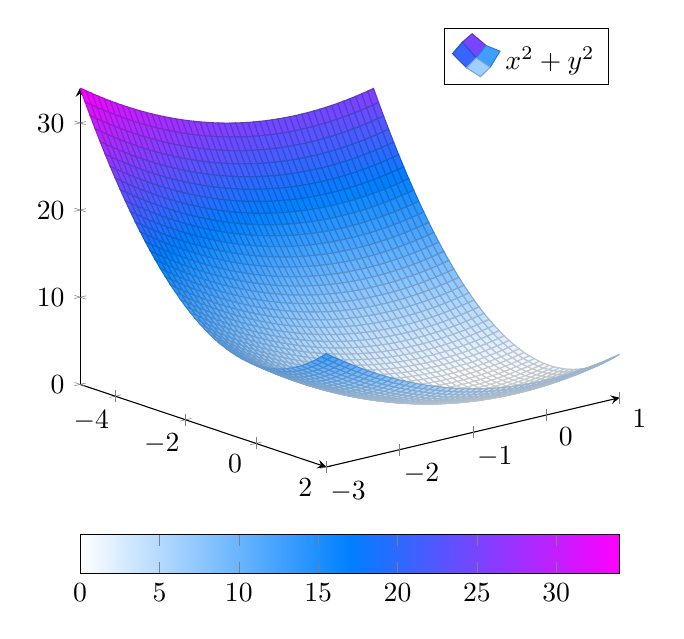
\begin{tikzpicture}
		\begin{axis}[colormap/cool, axis lines = left, colorbar horizontal, view = {50}{20}]
			\addplot3[
				surf,
				samples = 50,
				domain = -5:2,
				domain y = -3:1
			]
			{x^2+y^2};
			\addlegendentry{$x^2 + y^2$}
		\end{axis}
	\end{tikzpicture}
\end{center}

\subsection{\texttt{tcolorbox} Usage}
\begin{tcolorbox}[colback=red!5!white, colframe=red!75!black]
	\[ \int x\ \mathrm{d} x = \frac{1}{2} \cdot x^{2} + C \]
\end{tcolorbox}


% \begin{noindent}
\begingroup
  \raggedright
    \bibliographystyle{apacite}
    \bibliography{refs/refs.bib}
  \nocite{*}
\endgroup
% \end{noindent}

% \clearpage
% \appendix

\end{document}
